\section{Secretary Problem}
    
    \begin{frame}{Definition}
        
        \begin{center}
         	\uncover<+->{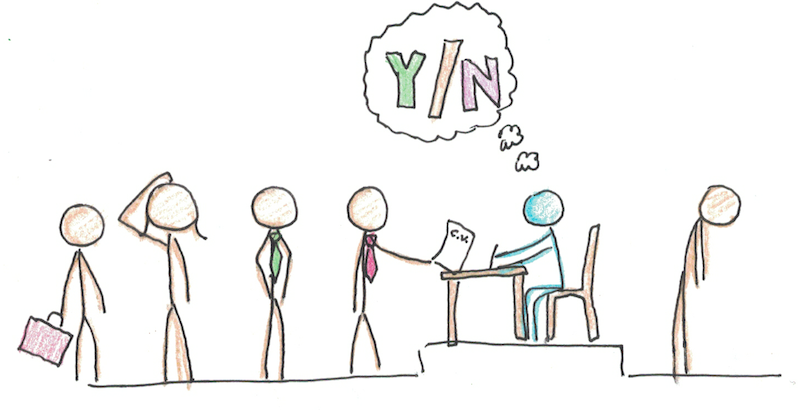
\includegraphics[scale=0.26]{pics/pic1.png}}
         	\end{center} 	
        \vspace{1pt}
        Want to hire THE best secretary!
        \begin{itemize}
        \uncover<+->{\item Single position to fill.}
        	\uncover<+->{\item n \textbf{rankable} candidates, one at a time, random order.}
        	\uncover<+->{\item No look-ahead, can't predict the future.}
        	\uncover<+->{\item No undo, can't call back candidates.}
        	
        \end{itemize}
    \end{frame}
    
    \begin{frame}{Policies}
        
       
        \begin{enumerate}

        	\uncover<+->{\item Choose the $r$th candidate.\\
        	Prob. of success: $\frac{1}{n}$. tends to zero as n tends to infinity.}
        	\vspace{5pt}
        	\uncover<+->{\item \textbf{Stopping Rule}: Observe until the $r$th candidate, accept best candidate afterwards.}
    
        \end{enumerate}
    \end{frame}
     \begin{frame}{Policies}
        
       
        \begin{itemize}

        	\item \textbf{Stopping Rule}: Observe until the $r$th candidate (reject all of them), accept best candidate afterwards.
         \begin{itemize}

        	\uncover<+->{\item Candidates $1$ to $r - 1$ are rejected.\\
        	Set $M$ the best candidate in $[1, r)$}
        	\uncover<+->{\item Pick first candidate after $r - 1$ that is better than $M$.}
        	 \end{itemize}
        	 \uncover<+->{It can be shown that the optimal strategy lies in this class of strategies.\cite{who}}
        \end{itemize}
    \end{frame}

    
     \begin{frame}{Deriving the Optimal Strategy}
        
        \uncover<+->{\[Pr(r) = \sum_{i = 1}^{n} Pr(i \, \text{is selected} \cap Pr(i \, \text{is the best})\]}
        \uncover<+->{\[ = \sum_{i = 1}^{n} Pr(i \, \text{is selected}\ |\ i \, \text{is the best})\,\cdot Pr(i \, \text{is the best})\]}
        \uncover<+->{\[ = \sum_{i = 1}^{n} Pr(i \, \text{is selected}\ |\ i \, \text{is the best})\, \cdot \frac{1}{n}\]}
        \uncover<+->{\[ = \sum_{i = r}^{n} Pr(\max_{j \in [1, r)} x_j =\max_{j \in [1, i)} x_j \ |\ i \, \text{is the best})\, \cdot \frac{1}{n}\]}
        
     
    \end{frame}
\begin{frame}{Deriving the Optimal Strategy}
        
        \uncover<+->{\[ = \sum_{i = r}^{n} Pr(\max_{j \in [1, r)} x_j =\max_{j \in [1, i)} x_j \ |\ i \, \text{is the best})\, \cdot \frac{1}{n}\]}
        \uncover<+->{\[ = \sum_{i = r}^{n} \frac{r - 1}{i - 1}\, \cdot \frac{1}{n}\]}
        \uncover<+->{\[ = \frac{r - 1}{n}\cdot\,\sum_{i = r}^{n} \frac{1}{i - 1} \]}
        
     
    \end{frame}
    
    \begin{frame}{Deriving the Optimal Strategy}
        \begin{theorem}
        Optimal cutoff in the stopping rule tends to $\frac{n}{e}$ as $n$ increases.
        \end{theorem}
        \begin{proof}
        \uncover<+->{For cutoff value r, probability of success is:
\begin{equation}\label{eq1}
        P(r) = \frac{r - 1}{n}\cdot\,\sum_{i = r}^{n} \frac{1}{i - 1} }
        \end{equation}  
        \uncover<+->{For large values of $n$, $x = \lim_{n \rightarrow \infty} \frac{r}{n} $ and $t = \lim_{n \rightarrow \infty} \frac{i}{n} $, \ref{eq1} is a Riemann approximation of an integral:}
        
        \end{proof}
        
     
    \end{frame}
\begin{frame}{Deriving the Optimal Strategy}
        \begin{theorem}
        Optimal cutoff in the stopping rule tends to $\frac{n}{e}$ as $n$ increases.
        \end{theorem}
        \begin{proof}
         
        \uncover<+->{For large values of $n$, $x = \lim_{n \rightarrow \infty} \frac{r}{n} $ and $t = \lim_{n \rightarrow \infty} \frac{i}{n} $, \ref{eq1} is a Riemann approximation of an integral:}
        \uncover<+->{
		\begin{equation}\label{eq2}
        P(x) = x\ \int_x^1 \dfrac{1}{t}\;\mathrm{d}t = - x\ln x 
        \end{equation}}
        \uncover<+->{Now to find the optimal $r$:
        \[P'(x) = -\ln x - 1 = 0 \Rightarrow x = \frac{1}{e}\]
        }
        \end{proof}
        
     
    \end{frame}

\subsection{Applications}
	\begin{frame}{Real-Life Applications}
	\begin{itemize}
	\item Apartment hunting! \cite{hprof} \cite{matguy}
	\\
	Estimated $n$, used secretary problem to limit the hunting time. \\
	Optimal result.
	\item \textbf{Kepler's Problem}(1611): Wanted to find a new wife!\\
	11 candidates, married the 5th one. Not sure about the objective or the algorithm.\cite{who}\\
	Apparently optimal result!
	\end{itemize}
	\end{frame}
	
	\begin{frame}{Spherical Cow}
	
	\begin{columns}[b]
    \column{.48\linewidth}
    
    \begin{itemize}
	\item Needs knowing the exact value of $n$ in advance.
	\item Assumes no other information about the candidates.
	\item No callbacks at all.
	\item Ranks sometimes not easily determined. 
	\item Hiring the second-best is as bad as hiring the worst.
	\end{itemize}
    \vspace{\fill}
    \vspace{\fill}
    \null
    \vfill\vfill
    \vspace{30pt}

    \column{.48\linewidth}
    \begin{figure}
         \centering
         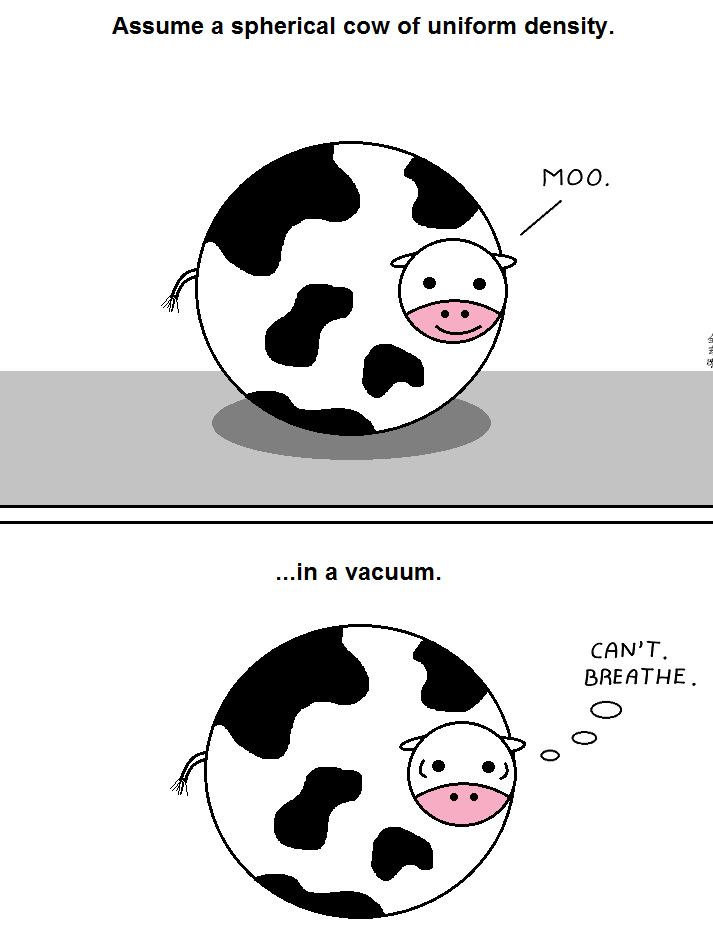
\includegraphics[scale=0.31]{pics/cow.png}
\caption{Spherical Cow}
    \end{figure}
    

\end{columns}
	
	
	
\end{frame}
\subsection{Variations}
\begin{frame}{How to Solve Them?}
	
	\begin{itemize}
	\uncover<+->{\item Needs knowing the exact value of $n$ in advance: \\}
	\uncover<+->{Suppose $n$ is a random variable with a known distribution.}

	\item No callbacks at all:\\
	\uncover<+->{Set a cost for each callback and minimize the overall cost.}

	\item Hiring the second-best is as bad as hiring the worst.
	\uncover<+->{\begin{itemize}
	\item Minimize rank: Average rank $O(1)$.\cite{optlec}
	\item Maximize payoff: cutoff at $\sqrt[2]{n}$, result tends to maximum at infinity.\cite{bguy}
	\end{itemize}}
	\end{itemize}
\end{frame}

\begin{frame}{Googol Game}
\uncover<+->{\begin{block}{Definition}
Ask someone to take as many slips of paper as she pleases, and on each slip write a different positive number. These slips are turned face down and shuffled. One at a time you turn the slips. The aim is to stop turning when you come to the number you guess is the largest of the series.
\end{block}}

\begin{itemize}
\uncover<+->{\item Two-person zero-sum game!}
\uncover<+->{\item Depends on how Alice chooses the numbers.}
\end{itemize}
\end{frame}


\begin{frame}{Models}
The difficulty of the problem changes depending on the information we know beforehand about the weights.\cite{mspra}
\begin{itemize}
\uncover<+->{\item \textbf{Full Information model}: Chosen i.i.d. from a known distribution.}
\uncover<+->{\item \textbf{Partial Information model}: Chosen i.i.d. from an unknown distribution.}
\uncover<+->{\item \textbf{Random Assignment model}: Adversary chooses weights, assigned using a uniform random one-to-one correspondence.}
\uncover<+->{\item \textbf{Zero information model}: Adversary assigns.} 
\end{itemize}
\end{frame}

